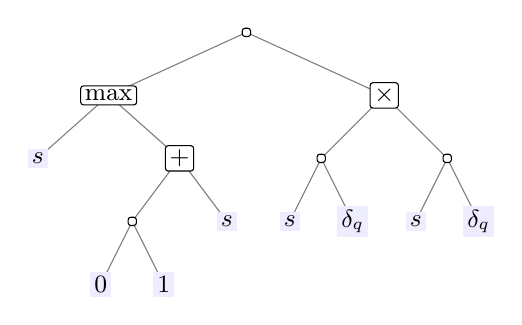
\begin{tikzpicture}[x=8mm,y=8mm,every node/.style={font=\small,inner sep=1.5pt}]
\draw[gray] (1.5,-3) -- (1,-4);
\draw[gray] (1.5,-3) -- (2,-4);
\draw[gray] (2.25,-2) -- (1.5,-3);
\draw[gray] (2.25,-2) -- (3,-3);
\draw[gray] (1.125,-1) -- (0,-2);
\draw[gray] (1.125,-1) -- (2.25,-2);
\draw[gray] (4.5,-2) -- (4,-3);
\draw[gray] (4.5,-2) -- (5,-3);
\draw[gray] (6.5,-2) -- (6,-3);
\draw[gray] (6.5,-2) -- (7,-3);
\draw[gray] (5.5,-1) -- (4.5,-2);
\draw[gray] (5.5,-1) -- (6.5,-2);
\draw[gray] (3.3125,0) -- (1.125,-1);
\draw[gray] (3.3125,0) -- (5.5,-1);
\node[fill=blue!7] at (0,-2) {$s$};
\node[fill=blue!7] at (1,-4) {$0$};
\node[fill=blue!7] at (2,-4) {$1$};
\node[draw,rounded corners=1pt,fill=white] at (1.5,-3) {$\AQ$};
\node[fill=blue!7] at (3,-3) {$s$};
\node[draw,rounded corners=1pt,fill=white] at (2.25,-2) {$+$};
\node[draw,rounded corners=1pt,fill=white] at (1.125,-1) {$\max$};
\node[fill=blue!7] at (4,-3) {$s$};
\node[fill=blue!7] at (5,-3) {$\delta_q$};
\node[draw,rounded corners=1pt,fill=white] at (4.5,-2) {$\AQ$};
\node[fill=blue!7] at (6,-3) {$s$};
\node[fill=blue!7] at (7,-3) {$\delta_q$};
\node[draw,rounded corners=1pt,fill=white] at (6.5,-2) {$\AQ$};
\node[draw,rounded corners=1pt,fill=white] at (5.5,-1) {$\times$};
\node[draw,rounded corners=1pt,fill=white] at (3.3125,0) {$\AQ$};
\end{tikzpicture}
